\documentclass[11pt,a4paper]{article}

\usepackage{fontspec}
\usepackage{geometry}
\usepackage{graphicx}
\usepackage{booktabs}
\usepackage{array}
\usepackage{xcolor}
\usepackage{hyperref}
\usepackage{amsmath}

\setmainfont{Arial}

\geometry{margin=2.2cm}
\hypersetup{
    colorlinks=true,
    linkcolor=black,
    urlcolor=blue
}

\definecolor{accent}{HTML}{2F6F73}
\definecolor{warning}{HTML}{B45309}
\definecolor{muted}{HTML}{5F6368}

\title{\textbf{A/B Test Analysis: New Landing Page Evaluation}}
\author{Portfolio case}
\date{}

\begin{document}
\maketitle

\section*{Executive Summary}

An e-commerce company tested a new landing page against the current page.
The goal of the experiment was to determine whether the new page increases user conversion.

The new page did not produce a statistically significant improvement.
The control group conversion rate was \textbf{12.04\%}, while the treatment group conversion rate was \textbf{11.88\%}.
The absolute effect was \textbf{-0.158 percentage points}, with a p-value of \textbf{0.190}.
The 95\% confidence interval for the effect was \textbf{[-0.394 pp; +0.078 pp]}.

\vspace{0.3cm}
\noindent
\textbf{Recommendation:} do not roll out the new landing page in its current form.

\section{Business Problem}

The experiment answers the following business question:

\begin{quote}
Does the new landing page increase user conversion compared with the old page?
\end{quote}

The primary metric is conversion rate:

\[
Conversion\ Rate = \frac{Converted\ Users}{Total\ Users}
\]

A positive and statistically significant effect would support a full rollout of the new page.
If the effect is not significant, the available evidence is not strong enough to replace the old page.

\section{Dataset}

The raw dataset contains \textbf{294,478} rows and 5 fields: user identifier, timestamp,
experiment group, landing page shown, and binary conversion flag.
The experiment ran from \textbf{2017-01-02} to \textbf{2017-01-24}.

\begin{table}[h]
\centering
\begin{tabular}{ll}
\toprule
\textbf{Field} & \textbf{Description} \\
\midrule
\texttt{user\_id} & Unique user identifier \\
\texttt{timestamp} & Time of experiment exposure \\
\texttt{group} & Experiment group: control or treatment \\
\texttt{landing\_page} & Page shown to the user: old\_page or new\_page \\
\texttt{converted} & Binary conversion flag: 0 or 1 \\
\bottomrule
\end{tabular}
\caption{Raw dataset structure}
\end{table}

\section{Data Cleaning}

Before estimating the effect, invalid rows were removed:

\begin{itemize}
    \item control users should see only \texttt{old\_page};
    \item treatment users should see only \texttt{new\_page};
    \item each user should be counted once.
\end{itemize}

\begin{table}[h]
\centering
\begin{tabular}{lr}
\toprule
\textbf{Metric} & \textbf{Value} \\
\midrule
Raw rows & 294,478 \\
Clean user-level rows & 290,584 \\
Removed invalid or duplicate rows & 3,894 \\
\bottomrule
\end{tabular}
\caption{Data cleaning result}
\end{table}

\section{Methodology}

A two-proportion z-test was used to compare conversion rates.

\textbf{Null hypothesis:}
\[
H_0: p_{treatment} = p_{control}
\]

\textbf{Alternative hypothesis:}
\[
H_1: p_{treatment} \neq p_{control}
\]

The treatment effect was calculated as:

\[
Lift = p_{treatment} - p_{control}
\]

Significance level: \(\alpha = 0.05\).

\section{Results}

\begin{table}[h]
\centering
\begin{tabular}{lrrr}
\toprule
\textbf{Group} & \textbf{Users} & \textbf{Conversions} & \textbf{Conversion Rate} \\
\midrule
Control: old page & 145,274 & 17,489 & 12.04\% \\
Treatment: new page & 145,310 & 17,264 & 11.88\% \\
\bottomrule
\end{tabular}
\caption{Conversion by experiment group}
\end{table}

\begin{figure}[h]
\centering
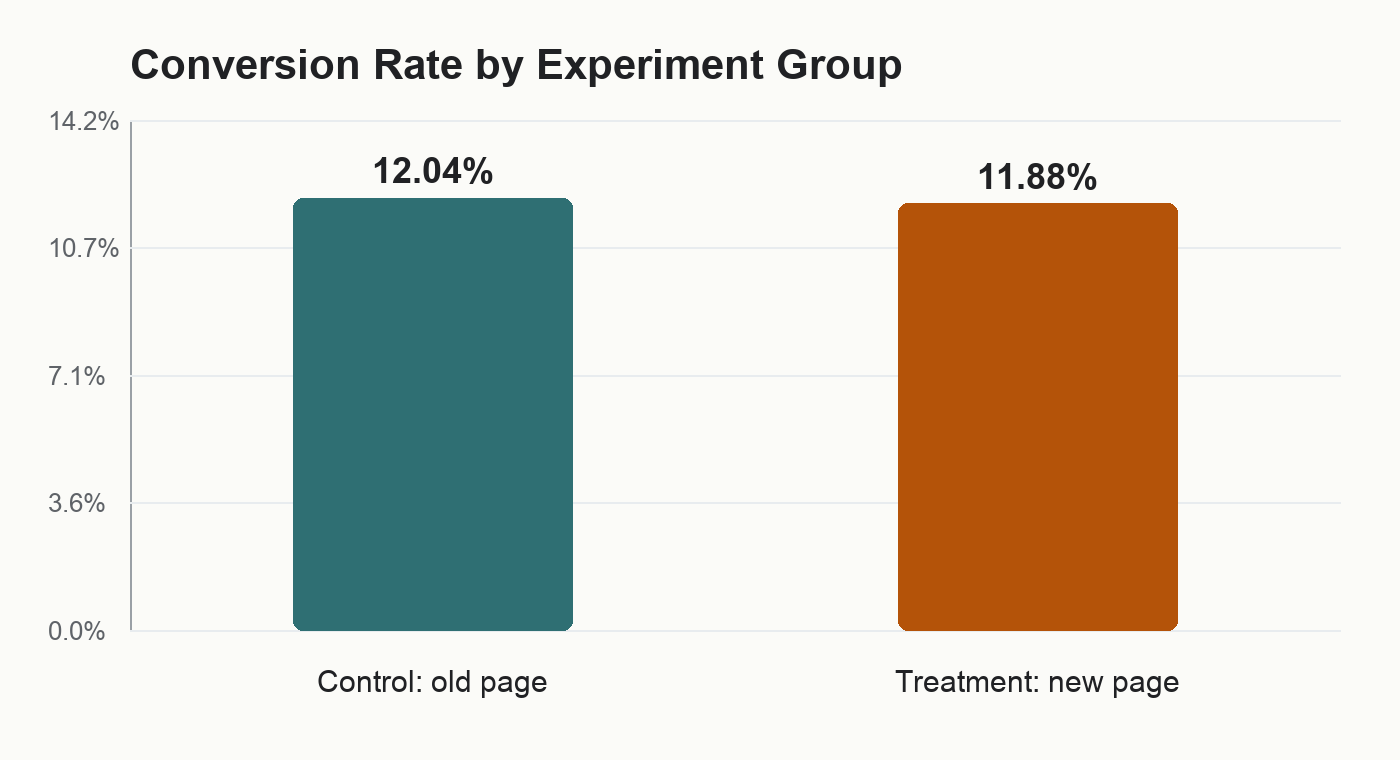
\includegraphics[width=0.94\textwidth]{../figures/report_conversion_rate_by_group.png}
\caption{Conversion rate by experiment group}
\end{figure}

\begin{table}[h]
\centering
\begin{tabular}{lr}
\toprule
\textbf{Metric} & \textbf{Value} \\
\midrule
Absolute lift & -0.158 pp \\
Relative lift & -1.31\% \\
z-score & -1.311 \\
p-value & 0.190 \\
95\% confidence interval & [-0.394 pp; +0.078 pp] \\
\bottomrule
\end{tabular}
\caption{Final statistical metrics}
\end{table}

\begin{figure}[h]
\centering
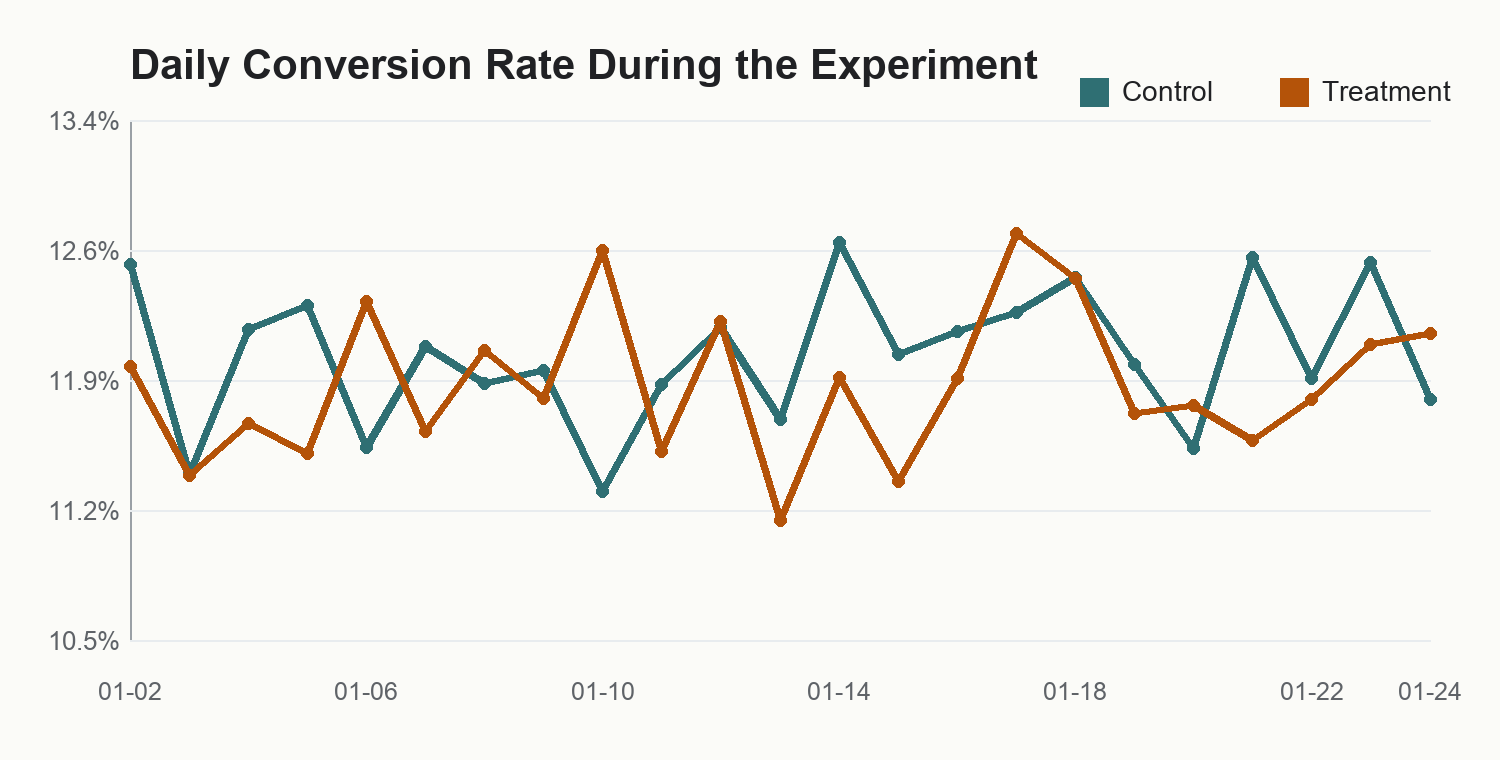
\includegraphics[width=0.98\textwidth]{../figures/report_daily_conversion_trend.png}
\caption{Daily conversion rate trend}
\end{figure}

\section{Interpretation}

The treatment group had a slightly lower conversion rate than the control group:
\textbf{11.88\%} versus \textbf{12.04\%}.
However, the p-value was \textbf{0.190}, which is above the 0.05 significance threshold.
The 95\% confidence interval also includes zero.

This means the observed difference may be explained by statistical noise.
Based on this experiment, there is not enough evidence to claim that the new landing page improves conversion.

\section{Recommendations}

\begin{enumerate}
    \item Do not roll out the new page to all users in its current form.
    \item Keep the old page as the default user experience.
    \item Review the new page design and identify likely friction points.
    \item Before the next test, define the minimum detectable effect and required sample size upfront.
    \item Analyze additional segments if business dimensions are available: device, traffic source, country, and new versus returning users.
\end{enumerate}

\section{Tools Used}

\begin{itemize}
    \item Python
    \item pandas
    \item manual two-proportion z-test
    \item LaTeX
    \item SVG visualizations
\end{itemize}

\end{document}
